\section{RollingLight design}

	% -TX
	% 	-modulation
	% 	-packet format
	% -RX
	% 	-led detection(multi)
	% 	-demodulation(yin vs fft)

	% -unsynchronization
	% 	-symbol delimiter
	% 	-seq_num
	% 	-parity
	% 	-實驗結果

\subsection{Rolling Shutter Frequency-Shift Keying (RS-FSK) }
\subsubsection{Modulation}
The fundamental idea of RS-FSK is to use the square waves of a number of different \textbf{frequencies} as different symbols, mapped to different bit patterns of the same length. The signal of the $i$-th symbol is represented by the fundamental frequency $f_i$ of the square wave:
\begin{equation}
	s_i(t)= I_{\max} \left \lceil \frac{\cos (2 \pi f_i t)}{2} \right \rceil
\end{equation} where $I_{\max}$ is the maximum output intensity of the transmitting light.

A frequency modulation is advantageous in the following aspects:
%\begin{itemize}
%\item
(1) The transmitted frequency can be demodulated by receivers with different sampling rate, as long as the sampling rate satisfies the Nyquist rate requirement. This implies that cameras with different read-out time are all compatible to a single transmission signal format.
(2) Demodulation is still possible when some segments of signal samples are lost in a symbol period, as long as the longest remaining signal segment has a length larger than the transmitted signal period. This addresses the time gap challenge previously described.
(3) The average intensity stays the same for all symbols, implying that the transmission is not observable by human eyes as long as the frequency is higher than 100 Hz.
%\end{itemize}

In addition, a square wave has some key properties which make it suitable for our purposes:
%\begin{itemize}
(1) It survives the moving average filtering mechanism due to the exposure operation, as long as the signal period is not an integer multiple of the exposure time. This is true even for very long exposure time. Most important of all, the fundamental frequency of the square wave remains the same and accurately observable after filtering.
(2) It is extremely simple and can be implemented with cheap microcontrollers or PWM driver chips. No DAC is needed to output signal at different amplitude levels.
(3) The modulation supports dimming by transmitting a modified square wave at the same frequency, but with different ratio of ON state and OFF state, i.e., duty cycle.
%\end{itemize}

\begin{figure}[!htb]
\centering
	\begin{subfigure}[h]{0.12\textwidth}
	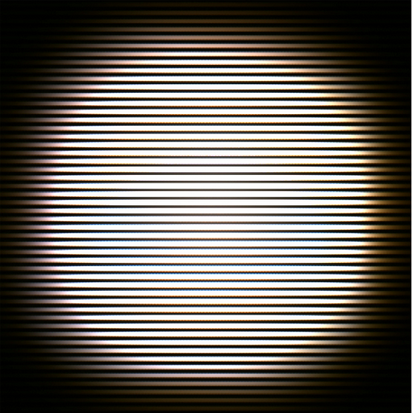
\includegraphics[width=\textwidth]{fig/strip1.png}
	\caption{8000 Hz}
	\end{subfigure}
	~	
	\begin{subfigure}[h]{0.12\textwidth}
	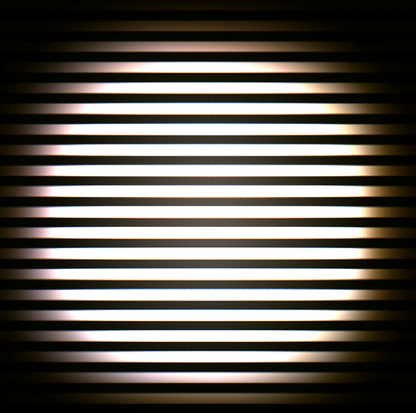
\includegraphics[width=\textwidth]{fig/strip2.png}
	\caption{4000 Hz}
	\end{subfigure}
	~	
	\begin{subfigure}[h]{0.12\textwidth}
	
\includegraphics[width=\textwidth]{fig/strip3.png}
	\caption{2000 Hz}
	\end{subfigure}
\caption{Received images of different transmitting frequencies.}
\label{fig:freq_strip}
\end{figure}
\autoref{fig:freq_strip} shows the received images of different transmitting frequencies.

\subsubsection{Demodulation}
\label{sec:period}
The transmitted signal period is the inverse of the transmitted signal frequency $f_i$. To obtain the \textbf{signal period}, we need to know the pixel width of strip in the received image first. In \autoref{fig:rx_strip}, as rows of pixels are sequentially obtained with sampling period $T_r$, one cycle of square wave transmission results in a pair of bright strip and dark strip in the image. The sum of whole widths is given by
\begin{equation}
W= \frac{1}{f_i T_r} \qquad \textrm{.}
\label{eq:widthtofreq}
\end{equation}

\begin{figure}[!htb]
	\centering
	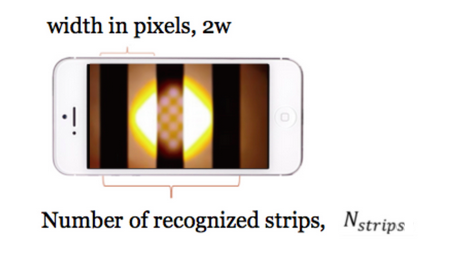
\includegraphics[scale=0.5]{fig/strip4.png}
	\caption{Received strips: w pixel}
	\label{fig:rx_strip}
\end{figure}

Note that the width of the bright strip could be larger than the width of the dark strip in the image. This is due to blooming, the overflow of charge from a saturated pixel into its neighboring pixel~\cite{el2005cmos}. We thus consider the widths of the bright strip and the dark strip together in the calculation, to average out the effect. Since $W$ might not be an integer, averaging the observed widths over a large image area would help to improve the accuracy of the estimate of the width. Then, the transmitted period $1/f_i$ can be calculated with \autoref{eq:widthtofreq}.

To have a more robust method to accurately determine the period of the signal, i.e., the average width of a pair of bright and dark strips in the image, we modified a well-known pitch detection algorithm (PDA), YIN~\cite{de2002yin}, that is originally designed to determine the fundamental frequency of a segment of audio signal in speech or music. We chose to use a method that operates in time domain, so that computationally expensive Fourier Transform operation can be avoided.

We start by summing up all pixels in each row
\begin{equation}
	I[y]=\sum^{X_{\max}}_{x=1} I[x][y] \qquad \textrm{,}
\end{equation}
obtaining a one-dimensional signal, where $I[x][y]$ is the intensity (luminance)\footnote{If the obtained image is in RGB instead of grayscale, it needs to be converted to obtain the luminance information.} of the pixel at location $(x,y)$ in the received image. This operation uses pixels in different columns for redundancy, averaging out noises that exists in different columns of pixel.

To find the period of the periodic signal presented in $I[y]$, a difference function may be constructed:
\begin{equation}
	d_\Delta(\delta)=\sum^{H/2-1}_{y=1} (I[y] - I[y+\delta])^2
\end{equation}
and we search for the values of $\delta$ that are closest to zero. Note that $\delta$ represents both the shift in space in number of pixels and the shift in time in multiples of read-out time of the camera. As pointed out in~\cite{de2002yin}, using the difference function instead of the standard autocorrelation function (ACF) can avoid a large portion of the error caused by change of amplitudes in the signal, causing by the change of luminance in different rows of pixels. An added advantage is that subtraction is computationally more efficient than multiplication.

Another possible source of error happens at small $\delta$ values, since when $\delta<\frac{1}{f T_r}$, the difference function could produce a large value due to the fact that we use square waves - there is no significant change of signal amplitude except at the sharp transitions. We instead use cumulative mean normalized difference function (CMNDF)~\cite{de2002yin} to mitigate this problem:
\begin{equation}
	d_\Delta'(\delta) =\begin{cases} 1, & \textrm{if\;} \delta=\{0,1\} \\
	d_\Delta(\delta) / \left [ (1/\delta) \sum^\delta_{j=1} d_\Delta(j) \right ] & \textrm{otherwise.} \end{cases}
\end{equation}
The function now starts from $1$ at $\delta=0$ and remains large with small $\delta$ values, and only drops below $1$ when $d_\Delta'(\delta)$ falls below average. The smallest local minimum in $d_\Delta'(0 \leq \delta \leq H/2-1)$ is then located and serves as the period estimate of the received signal.

Using CMNDF, the system can determine the period of the transmitted signal with a resolution of read-out time. However, as the period of the signal is not always an integer multiple of the read-out time, i.e., the sampling period, the output could results in error up to half of the read-out time. We again resort to the method proposed in~\cite{de2002yin} - to use parabolic interpolation to estimate the location of the actual minimum that could exist between samples. Assuming that $\hat{\delta}$ is the integer value that corresponds to the smallest minimum in $d_\Delta'(\delta)$, this method only needs three function values, $y_{-1}=d_\Delta'(\hat{\delta}-1)$, $y_{0}=d_\Delta'(\hat{\delta})$, and $y_{+1}=d_\Delta'(\hat{\delta}+1)$, to determine the new estimate:
\begin{equation}
	\hat{\delta}'=\hat{\delta}+\frac{y_{+1}-y_{-1}}{2 (2 y_0 - y_{+1} - y_{-1})}
\end{equation}
With parabolic interpolation, our modified YIN algorithm can very accurately determine the period of the transmitted signal. Note that the output of the algorithm is in pixel. It can be converted back to be in unit of time by multiplying the number with $T_r$.


\subsection{Problem Statement: Unsynchronized Transmitter and Receiver}

\subsubsection{The Problem}

As the transmitting light and the receiving camera are not synchronized, the transmitting frame rate and the receiving frame rate are usually not the same. 
As mentioned is~\cite{hu2013lightsync}, the received frame rate exhibits more variability for several reasons. For example, HTC One X camera appears to record videos are 24 fps, but the camera callback API can only support saving the frames at 15 to 20 fps. The callback slows down when there is insufficient memory available in the system. The frame rate on the Samsung Galaxy S III is only stable if the CPU is locked to its maximum frequency with its setCPU app. Otherwise, it fluctuates hugely between 21 to 29 fps for an entirely white foreground, and have an average of around 25 fps. Even when the frame rate appears steady, the inter-frame interval still varies.
In our design, we assume that the ratio $fps_{tx}$ / $fps_{rx}$ is not more than 2 or less than 0.9, which means the receive frame rate is between 15 and 33 fps when the transmitting frame rate is 30 fps. Note that this can be changed with straightforward modifications to our design to allow a larger variability of frame rate.

\textbf{Received frame patterns.} Given various potential combinations of the transmitting and receiving frame rates, we perform a simple experiment to study the received frame pattern. We transmit the data at several frame rates, and record the video with the PointGrey Flea3 camera~\cite{pointgrey_flea} with 30 fps.

\autoref{fig:diff_tx} shows the received frame pattern. For each received frame, we can detect which of the originally transmitted frames corresponds to it, and plot a circle for each detected frame. 

\begin{figure}[!htb]
   \centering
   \begin{subfigure}[h]{0.25\textwidth}
      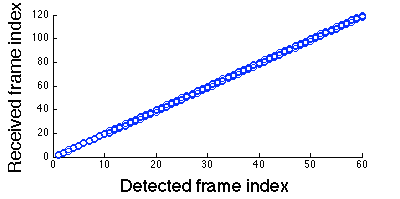
\includegraphics[width=\textwidth]{fig/tx_15.png}
      \caption{tx = 15 fps} \label{fig:tx_15fps}
   \end{subfigure}%
   ~
   \begin{subfigure}[h]{0.25\textwidth}
      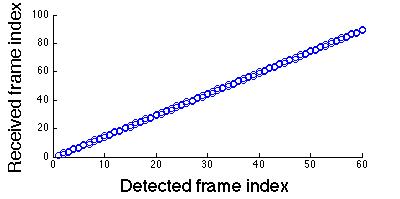
\includegraphics[width=\textwidth]{fig/tx_20.png}
      \caption{tx = 20 fps} \label{fig:tx_20fps}
   \end{subfigure}%
   \\   
   \begin{subfigure}[h]{0.25\textwidth}
      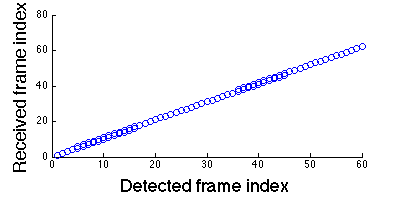
\includegraphics[width=\textwidth]{fig/tx_29.png}
      \caption{tx = 29 fps} \label{fig:tx_29fps}
   \end{subfigure}%
   ~
   \begin{subfigure}[h]{0.25\textwidth}
      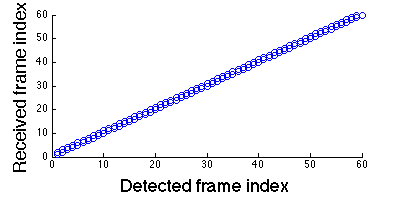
\includegraphics[width=\textwidth]{fig/tx_30_2.png}
      \caption{tx = 30 fps} \label{fig:tx_30fps_2}
   \end{subfigure}%
   \\
   \begin{subfigure}[h]{0.25\textwidth}
      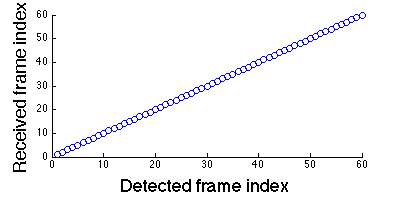
\includegraphics[width=\textwidth]{fig/tx_30.png}
      \caption{tx = 30 fps} \label{fig:tx_30fps}
   \end{subfigure}%
   ~   
   \begin{subfigure}[h]{0.25\textwidth}
      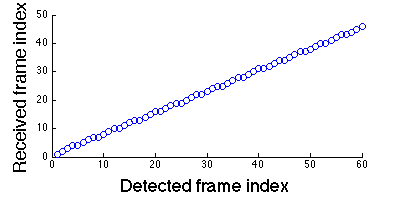
\includegraphics[width=\textwidth]{fig/tx_40.png}
      \caption{tx = 40 fps} \label{fig:tx_40fps}
   \end{subfigure}%
  \\
   \begin{subfigure}[h]{0.25\textwidth}
      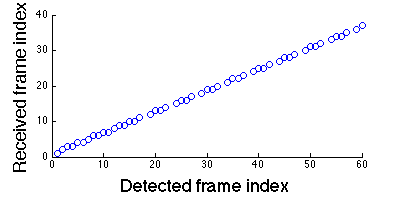
\includegraphics[width=\textwidth]{fig/tx_50.png}
      \caption{tx = 50 fps} \label{fig:tx_50fps}
   \end{subfigure}%
   ~
   \begin{subfigure}[h]{0.25\textwidth}
      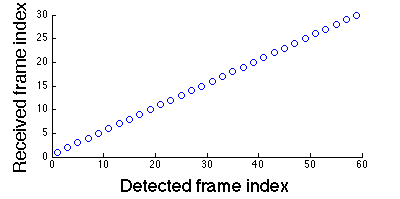
\includegraphics[width=\textwidth]{fig/tx_60.png}
      \caption{tx = 60 fps} \label{fig:tx_60fps}
   \end{subfigure}%
   \caption{Received frame patterns under different tx fps}
   \label{fig:diff_tx}
\end{figure}

When two or more detected frame indices correspond to the same received frame index, this captured frame contains a \textbf{mixture of two or more transmitted symbols}. When two or more received frame indices correspond to the same detected frame index, these captured frames have \textbf{redundant transmitted symbols}. Any gap between consecutive received frame indices indicates a \textbf{symbol loss}.

At 15 fps and 20 fps, we capture at least one complete frame with a full symbol. However, other frames show that the mixed frames and redundant frames are also possible due to random phase offsets.

When the transmitting rate is close to the receiving rate - 30 fps, mixed frames would be received for a few consecutive frames. Even when the transmitting frame rate is exactly 30 fps, mixed frames can still occur, in which case, it would always be the case received due to the constant phase offset, as shown in \autoref{fig:tx_30fps_2}. In the other case, a single transmitted symbol would always be received in each frame, as shown in \autoref{fig:tx_30fps}.

As the transmitting rate increases further, we start to experience mixed and missed symbols at times.

Since the camera records the videos at 30 fps, detecting the same number of transmitted frames requires receiving far more frames at a low transmitting rate. Therefore, the scales of the vertical axis are different across the subfigures of \autoref{fig:diff_tx}.

\subsubsection{The Probability}
\label{sec:unsync}
To figure out the symbol loss and mixed frame problems, we first want to know how often do they happen, thus we derive the probabilities under different conditions. In addition, we want to know what factors affect them and how to address them.

\textbf{Case I: When the transmitting frame rate is higher than the receiving frame rate,}
there could be symbol loss, defined as no part of the transmitting frame duration of a particular symbol is covered by the exposure time of any receiving image frame. 
\autoref{fig:miss} illustrates the missing symbols. 
Let the transmitting frame duration be $T_{f,tx}$ (symbol time), the receiving frame duration be $T_{f,rx}$, and the Y size of the image area illuminated by the transmitting light be $H$. The gray part is the time gap that the camera is not receiving the transmitting symbols. If $T_{f,tx} < T_{f,rx} - H T_r$, which means the transmitting symbols may appear in the gray part, then a symbol loss is possible. In that case, the probability of a symbol lost is given by
\begin{equation}
	P_{\operatorname{miss}}=\frac{T_{f,rx} - H T_r - T_{f,tx} }{T_{f,rx}} \qquad \textrm{.}
\end{equation}

We can see that the probability of the symbol loss in \autoref{fig:miss} is around 1/2, which means there is a symbol loss followed by every received symbol.

\begin{figure}[!htb]
  \centering
  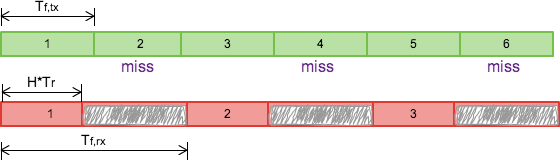
\includegraphics[scale=0.35]{fig/miss.png}
  \caption{Missing symbol illustration.}
  \label{fig:miss}
\end{figure}

A more common event which could happen when the transmitting frame duration and the receiving frame duration are different is that in a single image frame there could be multiple image areas each corresponding to a symbol. In other words, a mix of different symbols in a single receiving image frame. 
\autoref{fig:mix} illustrates the mixed frames. If the boundary between two consecutive transmitting symbols locates in the red part, during which the camera is receiving the transmitting symbols, then there is a mixed frame.
The probability for this event is given by
\begin{equation}
P_{\operatorname{mix}}=\begin{cases} \frac{H T_r}{T_{f,tx}}, & \textrm{if\;} T_{f,tx} \geq H T_r \\
1, & \textrm{otherwise.} \end{cases}
\end{equation}

We can see that the probability of the mixed frame in \autoref{fig:mix} is around 1/3.

\begin{figure}[!htb]
  \centering
  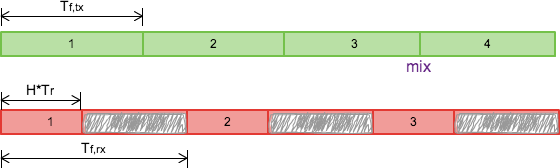
\includegraphics[scale=0.35]{fig/mix.png}
  \caption{Mixed frame illustration.}
  \label{fig:mix}
\end{figure}

A mixed frame is a very common and periodic event. Even when the transmitting and the receiving frame durations are very close to each other, mixed frames would be received for a few consecutive frames. After receiving a few frames with only a single symbol, consecutive mixed frame would appear again. \autoref{fig:mix_photo} shows the received frame with mixed symbols.
If the boundary of the image areas corresponding to different symbols is not determined, then the period detection algorithm would output one value. The value would usually be closer to the signal period of the symbol that occupies a larger image area, but usually has a large error. 

\begin{figure}[!htb]
  \centering
  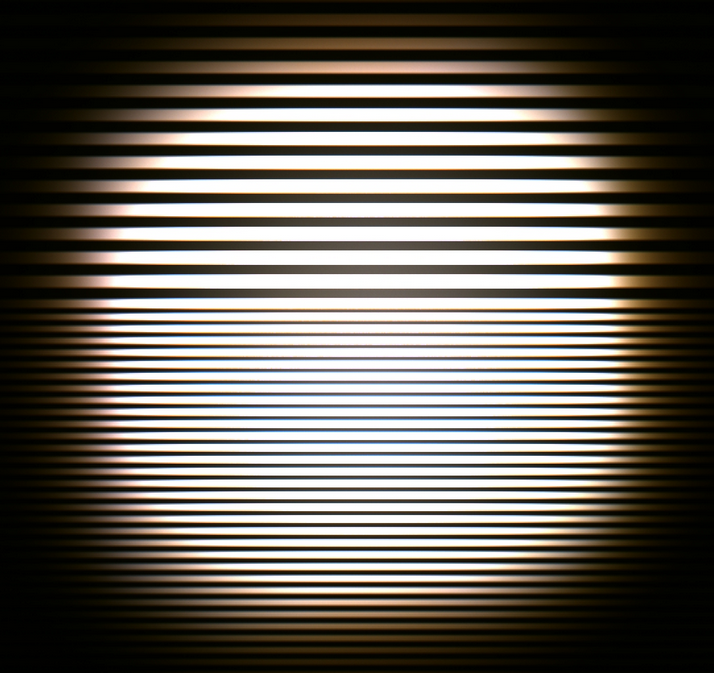
\includegraphics[scale=0.1]{fig/mix_photo.png}
  \caption{Received frame with mixed symbols.}
  \label{fig:mix_photo}
\end{figure}

\textbf{Case II: When the transmitting frame rate is lower than the receiving frame rate,}
a redundant symbol is possible. Although no information is lost, the receiver still needs to detect a redundant symbol so that it can be dropped to obtained the correct symbol sequence. 

\begin{figure}[!htb]
  \centering
  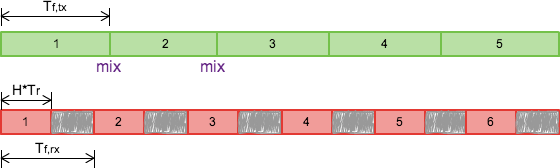
\includegraphics[scale=0.35]{fig/mix2.png}
  \caption{Mixed frame illustration.}
  \label{fig:mix2}
\end{figure}

On the other hand, a mixed frame is also possible in this case. The probability for a mixed frame is given by
\begin{equation}
P_{\operatorname{mix}}=\frac{H T_r}{T_{f,tx}} \qquad \textrm{.}
\end{equation}
which is same as the probability in Case I.
We can see that the probability of the mixed frame in \autoref{fig:mix2} is around 1/3.

According to the probability of lost symbol and mixed frame, the transmitting frame duration ($T_{f,tx}$), the receiving frame duration ($T_{f,rx}$), the height of the LED in the image ($H$), and the read-out time of camera sensor ($T_r$) and the factors which may affect the probabilities. We will introduce and evaluate how well our design address these issues in the following chapters.

\subsection{System Architecture and End-to-End System Flow}
\begin{figure*}[!htb]
	%\centering
	\hspace{-3em}
	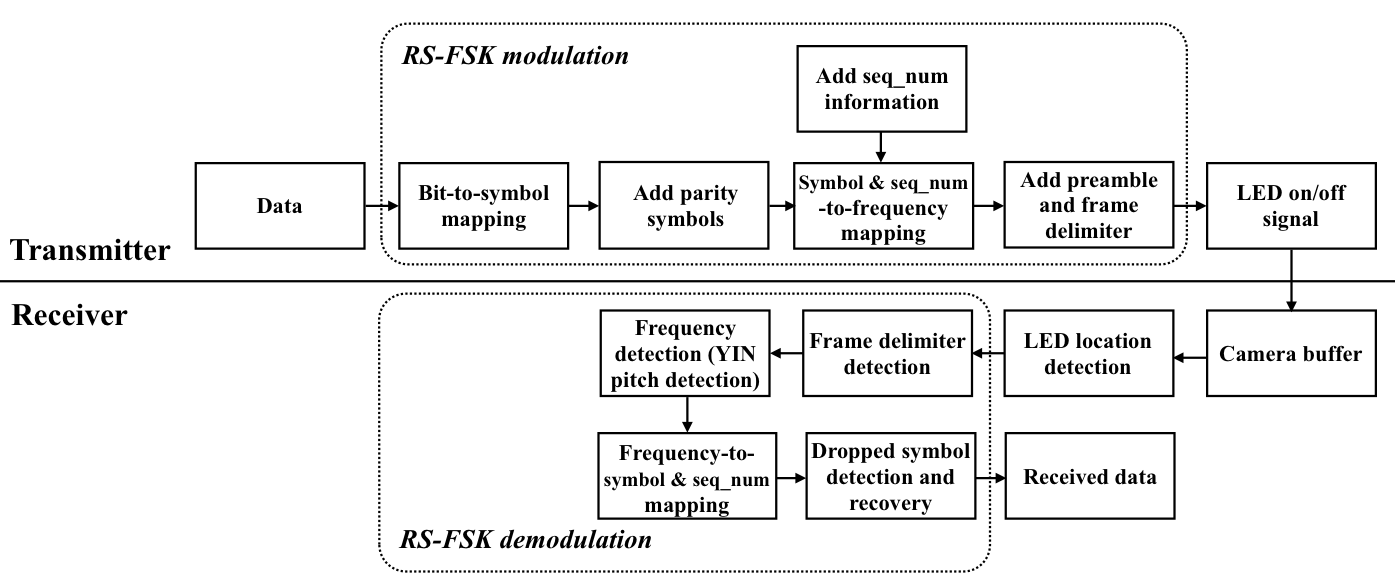
\includegraphics[scale=0.375]{fig/arch.png} 
	\caption{Block Diagram of our Proposed System}
	\label{fig:SystemArchitecture}
\end{figure*}

This section describes the overall end-to-end system flow.

\textbf{Bit-to-symbol mapping.} Data bits to be transmitted will first be split into bit patterns of a constant length. Each bit pattern is then mapped to a data symbol.

\textbf{Parity symbol.} As symbols could be lost or corrupted due to the time gap of the channel or if the exposure time is an integer multiple of the signal period,
a parity symbol is inserted for every $n$ data symbols by \textbf{XOR-ing} all $n$ data symbols, so that if only one of the $n$ data symbols or the parity symbol is not correctly received, the receiver can \textbf{recover the lost symbol}. The number of parity symbols that should be added to a packet can be determined by calculating expected number of lost symbols in a packet using the probability equation in \autoref{sec:unsync}.

\textbf{Sequence number.} After constructing a sequence of symbols, including the parity symbol, to be transmitted, we label each symbol with a \textbf{1.5 bit} sequence number $=\{0,1,2\}$.
The sequence number can be obtained by calculating the index number modulo 3.
The sequence number is then combined with the data symbol to become one meta symbol, then mapped to one of the selected signal periods.
Note that the sequence number reduces the number of bits that can be represented by each symbol by 1.5 bits. However, this is required to detect \textbf{lost symbols} (when the transmitting frame duration is smaller than the receiving frame duration) or \textbf{redundant symbols} (when the transmitting frame duration is larger than the receiving frame duration).
Taking the assumption into consideration, it can be proved that there could be no consecutive symbol losses. Thus, a 1.5 bit sequence number, $\{0,1,2\}$, would be sufficient determine the location of a lost symbol in the sequence. 
Note that the sequence number will be represented by the most significant 1.5 bits in a symbol, i.e., symbols with different sequence numbers will be separated with a large margin, and thus getting an erroneous sequence number is unlikely.

\textbf{Preamble symbol.} Next, the preamble symbol, which has a signal period known to the receiver, is inserted at the beginning of the symbol sequence.
The preamble symbol serves two functions: one is for the receiver to detect the start of the packet and start the subsequent demodulation process, while the other is for the receiver to accurately \textbf{calibrate its $T_r$ value} based on the period estimate of the preamble, so that the error of the period estimates of all subsequent symbols in this packet can be minimized. As a result, the signal period with the smallest error variation is selected as the period for the preamble symbol. In our experiment, we select the 5657.3886 Hz as the period for the preamble symbol. This is the highest frequency used in our design. 

\textbf{Symbol delimiter.} Finally, another signal period is selected as the symbol delimiter signal period.
In order to easily \textbf{separate consecutive symbols} in the same image, i.e., two areas in the image showing signals with different periods, a signal with this signal period will be transmitted for a short duration between any two symbol transmissions. %as Figure~\ref{fig:FD} shows. 
The transmitting light is then driven to transmit a sequence of square waves according to pre-determined list of signal periods representing the entire data packet.

% \begin{figure}[!htb]
%   \centering
%   \includegraphics[scale=0.8]{fig/fd.png} 
%   \caption{Frame delimiter illustration. The upper shows the frame without frame delimiter; the lower shows the frame with frame delimiter.}
%   \label{fig:FD}
% \end{figure}

\begin{figure}[!htb]
  \centering
  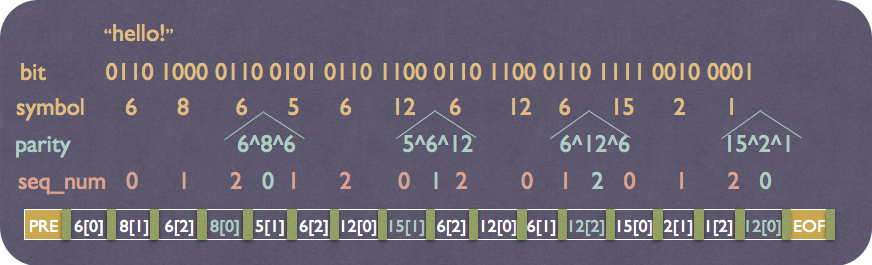
\includegraphics[scale=0.25]{fig/flow_tx.png} 
  \caption{An example flow of the transmitter end.}
  \label{fig:flow_tx}
\end{figure}

\autoref{fig:flow_tx} shows an example flow of the transmitter end. The message "hello!" is converted to the bit string, Then every 4-bit is mapped to a symbol. Assume the $P_{miss}$ is 0.25, which means a parity symbol is inserted for every 3 symbols. Next step we tag the symbols (including parity symbol) in the order of $\{0,1,2\}$ as the sequence number. The last step is to add the preamble symbol and the EOF symbol (the yellow part in the figure) at the beginning and the end of the data, and the symbol delimiter symbol (the green part in the figure) between each data symbols. 

\textbf{LED location detection.} The receiving camera captures a series of images with the transmitting light. The receiver starts the demodulation process by determining the image area occupied by the transmitting light. In our system, this is done by extracting an area with very high intensity values. More sophisticated detection and tracking algorithms based on computer vision techniques can be utilized if necessary.

\textbf{Symbol delimiter detection.}
A symbol delimiter detector is then executed to determine whether a symbol delimiter area presents in the image. \autoref{fig:flow_rx} shows the received image which contains a symbol delimiter. The detection step is done by calculating the value of the difference function described in \autoref{sec:period} for all possible symbol delimiter locations in the image, but only with a fixed shift value that equals the the signal period of the symbol delimiter. If the minimum value of the function for all possible delimiter locations is larger than a pre-defined threshold, then it will output the location of the symbol delimiter. Then, the period detection algorithm can be executed to determine the signal periods of two image areas separated by the symbol delimiter. In this case, the signal periods of both symbols can be accurately estimated.

% \begin{figure}[!htb]
%   \centering
%   \includegraphics[scale=0.25]{fig/FD_illustration} 
%   \caption{Received frame with frame delimiter.}
%   \label{fig:FD_photo}
% \end{figure}
\begin{figure}[!htb]
  \centering
  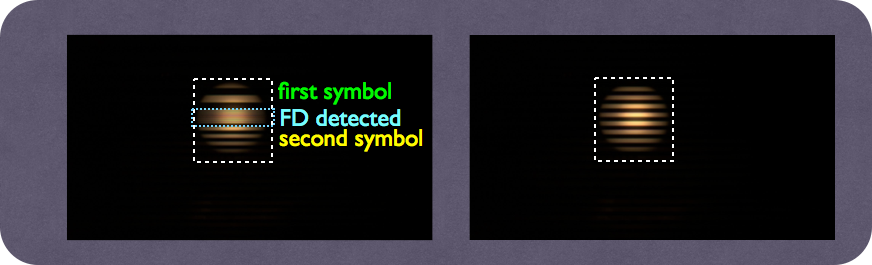
\includegraphics[scale=0.25]{fig/flow_rx.png} 
  \caption{An example flow of the symbol delimiter detection of the receiver end.}
  \label{fig:flow_rx}
\end{figure}

The estimated signal period will be mapped to a meta symbol. The meta symbol is then split into a sequence number and a data symbol.

\textbf{Dropped symbol detection and recovery.}
Then, the sequence number is used to identify any missing symbol or redundant symbol. Missing symbols will be reconstructed with corresponding parity symbols, while redundant symbols with the same sequence number will be dropped. In the case that redundant symbols with the same sequence number is demodulated to different symbols, the one decoded with the largest image area will be used.

The data string is finally obtained after mapping the sequence of data symbols back to the bit patterns, forming the original bit stream.

\subsection{System Components}

\begin{figure}[!htb]
  \centering
  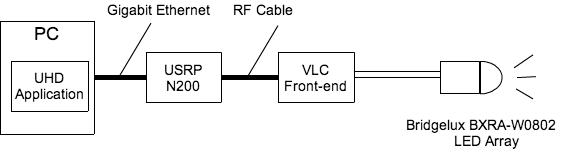
\includegraphics[scale=0.4]{fig/tx_component.png} 
  \caption{Transmitter Components}
  \label{fig:tx_component}
\end{figure}


As the system is still under development, the developed system should be sufficiently flexible so that it is easy to change various desires of the system, e.g., the modulation format, the protocol design, etc. 
To this end, we utilize a software-defined radio (SDR) platform in our system, which enables us to make most necessary modifications in software with minimal efforts. 
Additional hardware components were developed to interface between the SDR and the optical transmitting and receiving components. 
\autoref{fig:tx_component} shows the transmitter components in our proposed VLC system. 

In the transmitting end, we use a PC with USRP Hardware Driver (UHD) application to modulate the digital information in a packet into analog signal, in the format of digitized samples. 
The SDR is connected to the PC via gigabit Ethernet. The SDR converts the digitized samples sent from the PC into analog signal. 
The VLC front end board converts the voltage varying signal to current varying signal and outputs that to the LED. The signal would determine the output intensity of the LED. 

In the receiving end, we just use a camera to receive the optical signal and use simple computer vision and digital image processing mechanism to demodulate. We use PointGrey Flea3 camera~\cite{pointgrey_flea}, which provides the capability to manually control various camera parameters. We also use a number of smartphones to compare their performance.

In the following, we will describe the components in the system in detail.

\begin{figure}[!htb]
\centering
 \begin{subfigure}[h]{0.1\textwidth}
  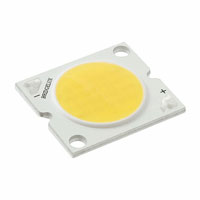
\includegraphics[width=\textwidth]{fig/LED_array.jpg} 
  \caption{Bridgelux BXRA-W0802 LED Array} \label{fig:led_array}
 \end{subfigure}
~
 \begin{subfigure}[h]{0.1\textwidth}
  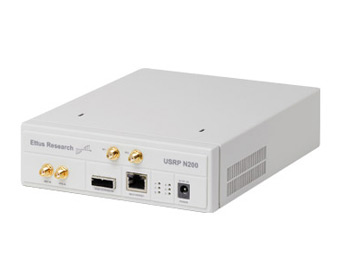
\includegraphics[width=\textwidth]{fig/usrp.jpg} 
  \caption{USRP N200 Software Defined Radio} \label{fig:usrp}
 \end{subfigure}
~
 \begin{subfigure}[h]{0.1\textwidth}
  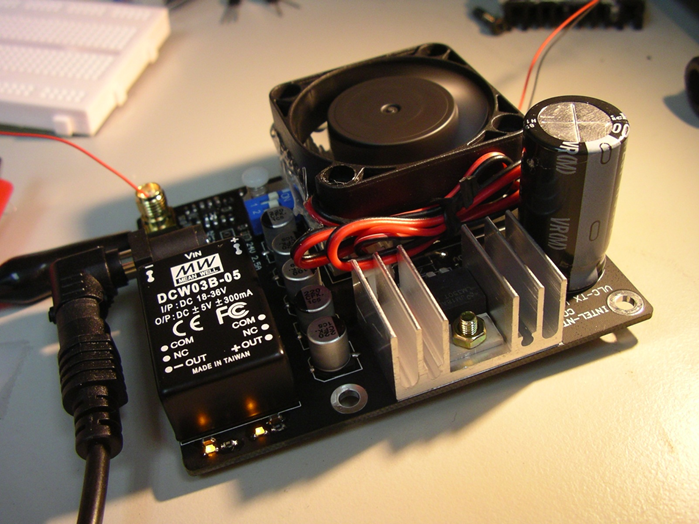
\includegraphics[width=\textwidth]{fig/VLC2_0.png} 
  \caption{VLC 2.0 Front-end Board} \label{fig:VLC_frontend}
 \end{subfigure}
\caption{Photos of Transmitter Components}
\label{fig:tx_photo}
\end{figure}

\begin{figure}[!htb]
\centering
 \begin{subfigure}[h]{0.2\textwidth}
  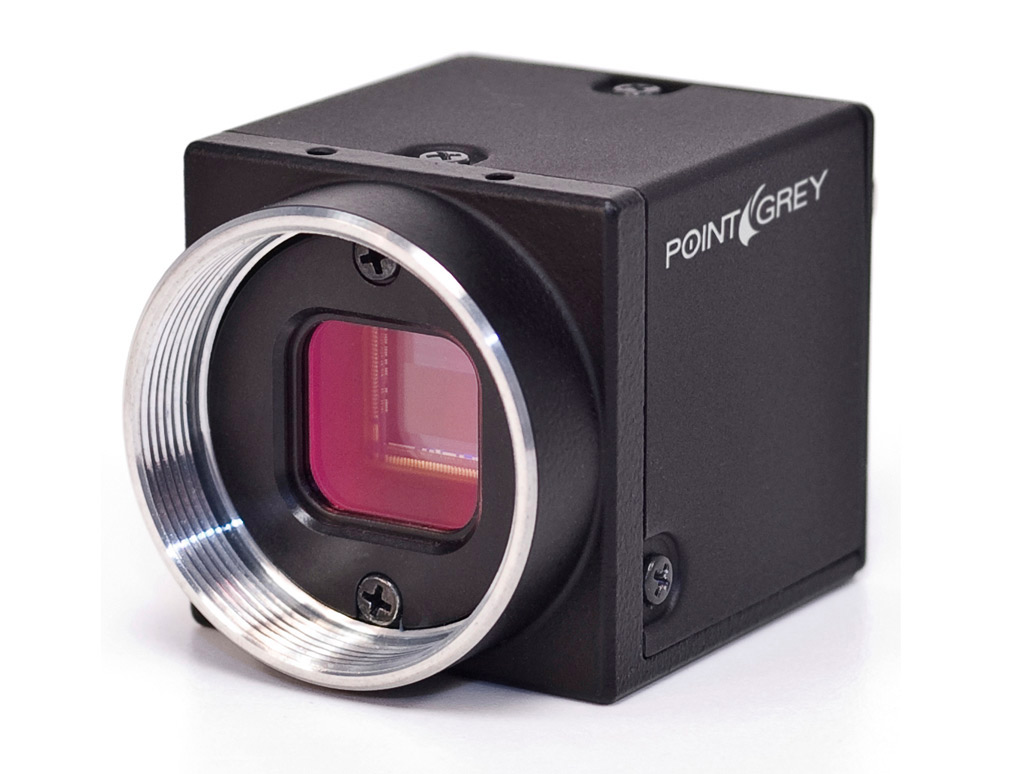
\includegraphics[width=\textwidth]{fig/flea3.jpg} 
  \caption{PointGrey Flea3 Camera} \label{fig:flea}
 \end{subfigure}
~
 \begin{subfigure}[h]{0.2\textwidth}
  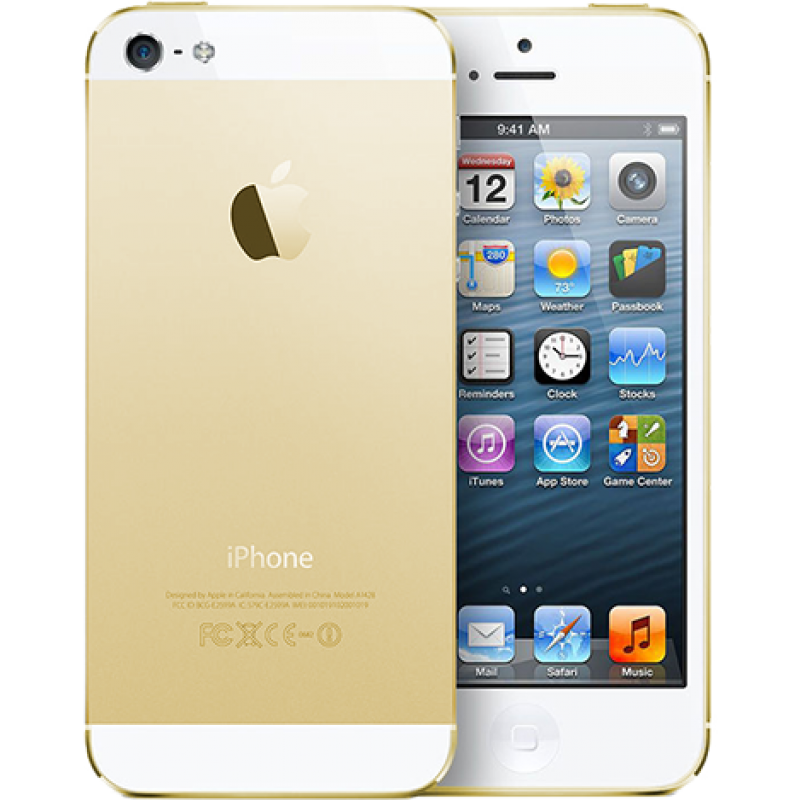
\includegraphics[width=\textwidth]{fig/iphone5s.png} 
  \caption{SmartPhone Camera (iPhone5S)} \label{fig:iphone5s}
 \end{subfigure}
\caption{Photos of Receiver Components}
\label{fig:rx_photo}
\end{figure}

\subsubsection{LED Array}
\autoref{fig:led_array} shows the Bridgelux BXRA-W0802~\cite{Bridgelux}, which is a high brightness LED array suitable for indoor illumination purposes and chosen as the transmitting LED component. The maximum DC forward current is 2 amps, and the typical forward voltage is around 13 volts, resulting in a maximum output power of 26 W. Typical luminous flux with 1050 mA forward is 850 lumen.

\subsubsection{Software Defined Radio}
As a highly flexible tool to realize the traditional RF communications, SDR has become our preferred platform to develop the VLC system. In our system, we use Ettus Universal Software Radio Peripheral (USRP) N200, as \autoref{fig:usrp} shows. USRP then converts the digital signal samples to analog voltage-varying signal.
The unit features a gigabit ethernet interface to transfer signal samples to the PC. 
N200 provides high-bandwidth and high-dynamic range processing capability. 
A modular design allows the N200 to operate from DC to 6 GHz. 

In our system we use a daughter board (LFTX) that is capable of transmitting signals from DC to 30 MHz. 
N200 can stream up to 50 MegaSample/s to and from host applications, and users can implement custom functions in the FPGA fabric, or in the on-board 32-bit RISC softcore. The FPGA offers the potential to process up to 100 MHz of RF bandwidth in both the transmit and receive directions. 
This is more than sufficient for our application as VLC usually operates in the range of 0.1 kHz to several kHz. The sampling rate to convert the digital samples to analog signal is configured at 1 MHz. This could emulate the clock rate of a low-cost microcontroller. Inaccuracy in the transmitted signal period could be caused by low sampling rate.

\subsubsection{UHD}
UHD is a driver developed by Ettus Research and is compatible with all USRP software-defined radios. 
UHD allows development on multiple operating systems.
UHD provides an application programming interface (API), which provides access to various functions of the USRP including synchronization, sample streaming, and configuration. 

In the thesis, we modify one of the example applications provided with the UHD software package to modulate the transmitting signals.

\subsubsection{VLC Front-end Board}

The output light intensity of the LED depends on the magnitude of the input current. Thus, a hardware component is required to interface between the SDR and the LED component, linearly converting a voltage-varying signal to a current-varying signal. We utilize a custom-made VLC front-end circuit board, as shown in \autoref{fig:VLC_frontend}. 

One of the main objectives for the design of the front-end board is to accurately convert the level of voltage in the input signal to the level of the output intensity of the attached LED. 
For example, when the voltage of input signal is zero, the front-end would control the light intensity of the LED to be zero, and when the voltage of the input signal is raised to the maximum, the light intensity of the LED should also at its maximum. 

Moreover, this conversion also needs to be done fast enough so that a high frequency signal can be transmitted. 

\subsubsection{Rolling Shutter Camera}
There are a number of cameras used in our experiments. 
 \autoref{fig:flea} shows the specification of PointGrey Flea3 (FL3-U3-88S2C-C)~\cite{pointgrey_flea}, a high-speed camera built for experimental purposes, thus various parameters such as exposure time can be adjusted to a wide range of values. This allows us to examine system performance in different conditions. 
 \autoref{tab:flea_spec} lists the specification of Point Grey Flea3 camera.

The cameras on smartphones, such as HTC New One and iPhone 5S shown in \autoref{fig:iphone5s} , are also selected for some experiments, in order to determine the expected performance of RS-FSK on cameras in off-the-shelf smartphones. 

\begin{table}[!htb]
\centering
\caption{Specification of Point Grey Flea3 (FL3-U3-88S2C-C).}
  %\large
	\begin{tabular}{lc}
  \hline Parameter & Value \\
  \hline 
	\hline Camera Sensor Format & 1/2.5" \\
	\hline Type of Sensor & Sony IMX121 CMOS \\
	\hline Pixel (H x V) & 4096 x 2160, 2048 x 1080 \\
	\hline Pixel Size (H x V) & 1.55$\mu$m x 1.55 $\mu$m \\
	\hline Max Frame Rate (fps) & 21.6, 60 \\
	\hline Type of Shutter & Rolling Shutter \\
	\hline Exposure Time & 0.015 ms - 1 s \\
	\hline Estimated Read-out Time & 0.01473 ms \\
  \hline 
	\end{tabular}
	\label{tab:flea_spec} 
\end{table}
